\subsubsection{Set Availability}
\begin{figure}[H]
    \centering
    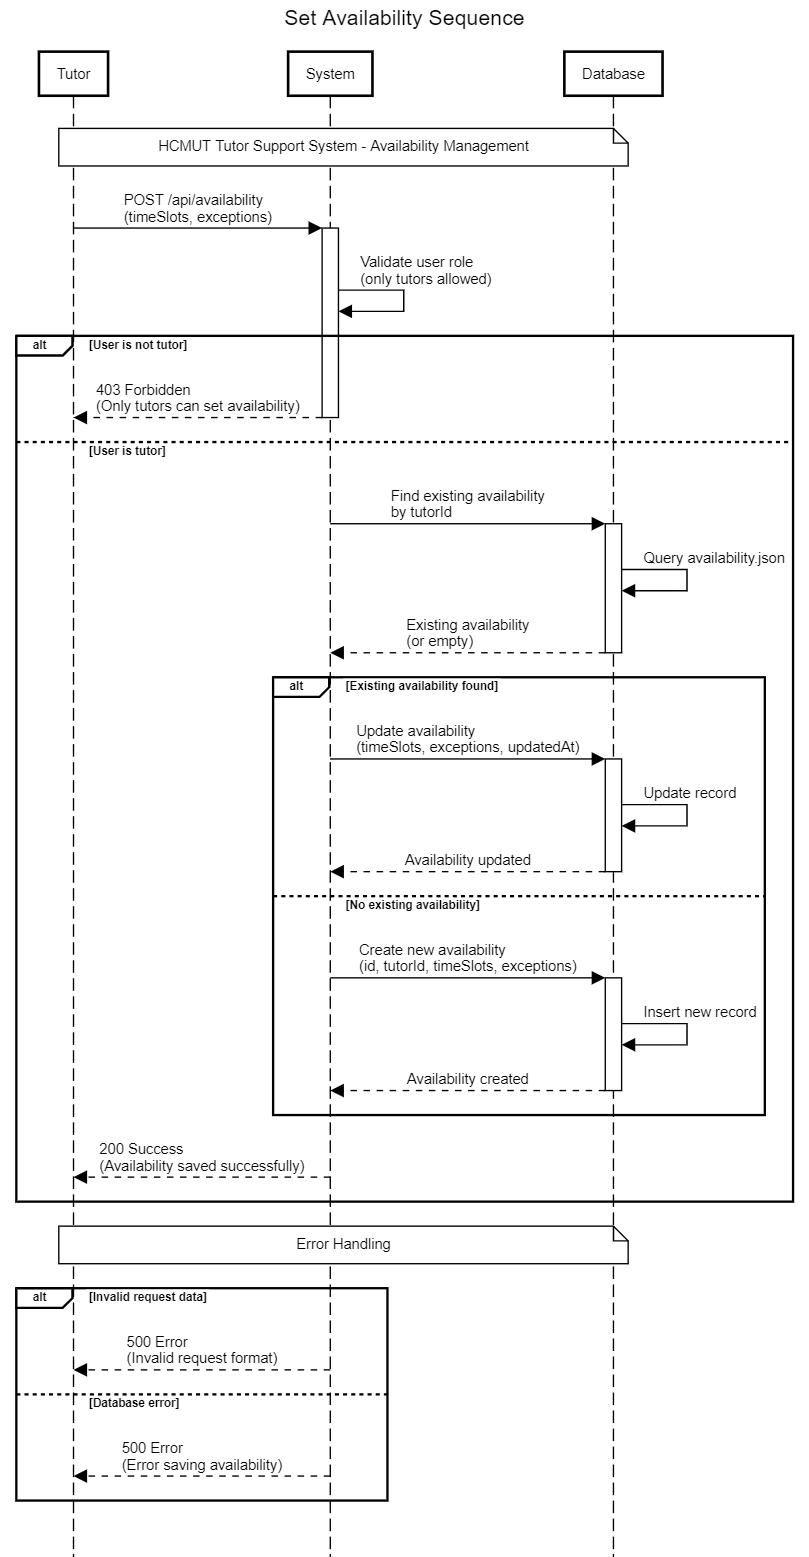
\includegraphics[width=0.6\textwidth]{graphics/chapter3/tutor/SetAvail.png}
    \caption{Sequence diagram of Set Availability}
    \label{fig:set_availability}
\end{figure}

\newpage
\noindent \textbf{Description} \\ 

\textbf{Actors:} Tutor, System, Database

\begin{enumerate}
    \item Tutor sends POST request to System with time slots and exceptions data
    \item System validates user role (only tutors are allowed to set availability)
    \item If user is not a tutor, System returns 403 Forbidden error to Tutor
    \item If user is a tutor, System queries Database to find existing availability by tutorId
    \item Database searches availability.json and returns existing availability (or empty if none exists)
    \item If existing availability is found:
    \begin{itemize}
        \item System updates the existing availability record with new time slots and exceptions
        \item Database modifies the record and confirms update to System
    \end{itemize}
    \item If no existing availability is found:
    \begin{itemize}
        \item System creates a new availability record with tutorId, time slots, and exceptions
        \item Database inserts the new record and confirms creation to System
    \end{itemize}
    \item System returns 200 Success response to Tutor confirming availability has been saved
    \item Error Handling: If invalid request data or database error occurs, System returns 500 Error to Tutor
\end{enumerate}


